\section{RFFT(Rule-Following Fine-Tuning)}

\subsection{RFFT 的步骤}


\begin{frame}
	\begin{columns}
		\begin{column}{.7\textwidth}
			\begin{figure}[t]
				\centering
				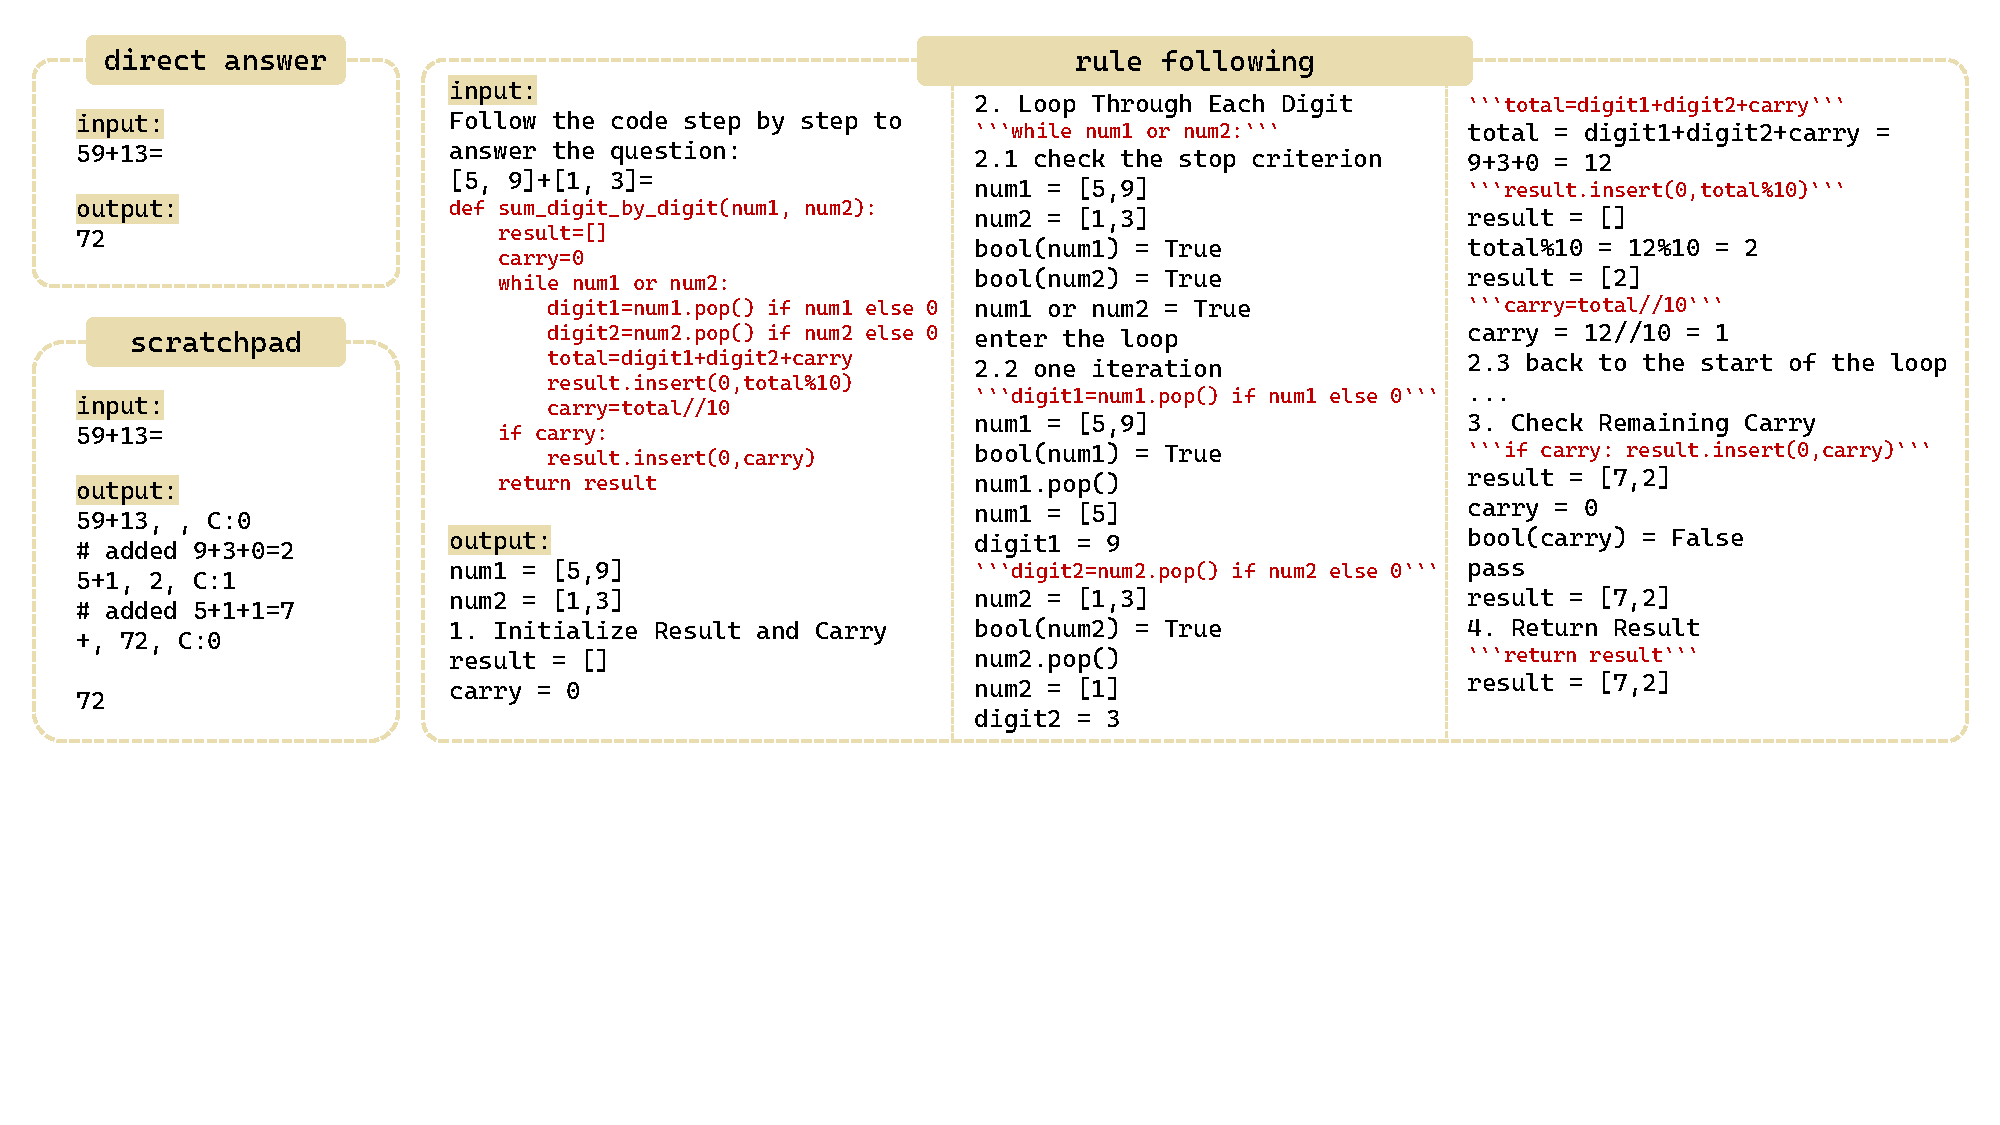
\includegraphics[width=\textwidth]{pic/prompt_new.pdf}
				\vspace{-5pt}
				\caption{Examples of input-output sequence of question $59+13$}
				\label{prompt}
			\end{figure}
		\end{column}
		\begin{column}{.3\textwidth}
			Step 1: Explicitly list the rules for solving a given task in the input.\\[0.2cm]

			Step 2: Finetune the model to follow the rules step by step.\\[0.2cm]

			可以有不用的方式阐述规则,including programs, pseudo-code, first-order logic, natural language, etc.
		\end{column}
	\end{columns}
\end{frame}

\subsection{RFFT 结果分析}
\begin{frame}{RFFT 结果分析} \begin{columns} \begin{column}{.7\textwidth} \begin{figure}[t] \centering \begin{subfigure}[t]{.45\textwidth} \centering 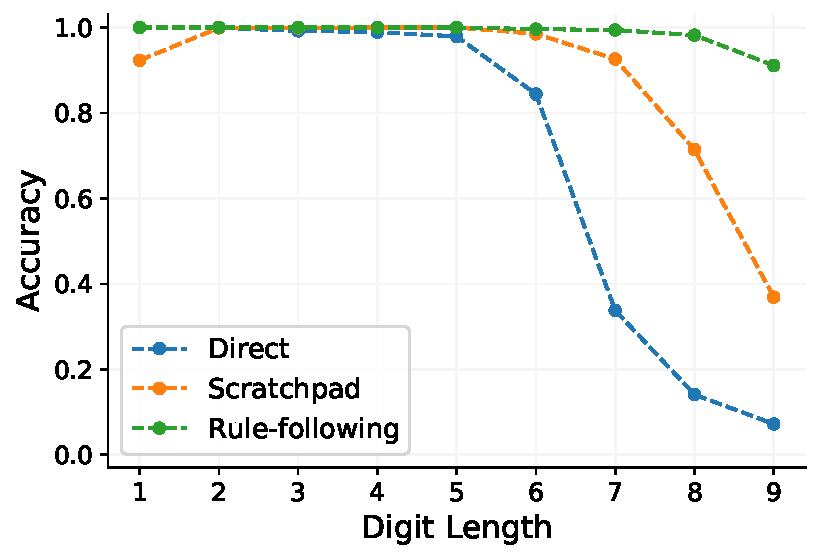
\includegraphics[width=\textwidth]{pic/llama_ft.pdf} \caption{Accuracy of Llama-7B fine-tuned with three methods tested on addition with 1-9 digits.} \label{fig:llama_ft} \end{subfigure}
				\hfill
				\begin{subfigure}[t]{.45\textwidth} \centering 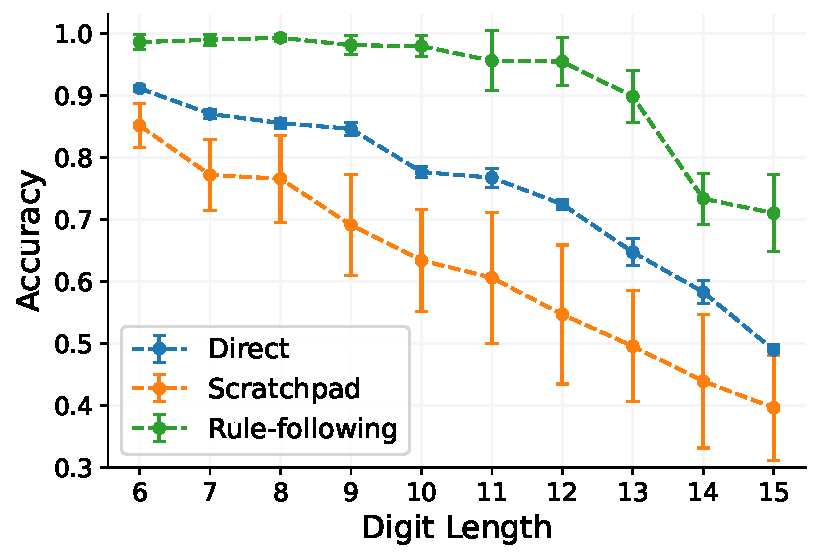
\includegraphics[width=\textwidth]{pic/gpt3_ft.pdf} \caption{Accuracy of GPT-3.5 fine-tuned with three methods tested on addition with 6-15 digits.} \label{fig:gpt3_ft} \end{subfigure}
				\caption{Accuracy of Llama-2-7B and GPT-3.5-turbo fine-tuned with direct answer, scratchpad and rule following on addition.}
				\label{fig:rfft}
				\vspace{-5pt}
			\end{figure}
		\end{column}
		\begin{column}{.3\textwidth} Llama-2-7B: RFFT: 91.1\% acc with 9-digit sums\\[0.2cm] scratchpad: less than 40\% acc\\[0.2cm] GPT-3.5-turbo: over 95\% acc on 12-digit addition (only 100 training samples) \end{column}
	\end{columns}
\end{frame}

\subsection{误差分析}
\begin{frame}{误差分析}
	\begin{itemize}
		\item RFFT 并不能带来100\%的准确性,作者发现大模型在计算时的每一步总能找到正确的规则,但是在一些基本的运算中会出现失误的现象,这可能是由于大模型幻觉或者是大模型处理长文本的局限性。\\[0.4cm]
		      \pause
		\item RFFT as a Meta Learning Ability:stronger models indeed need less examples to learn rules.\\[0.4cm]
		      \pause
		\item Given detailed rules, LLMs have certain abilities to follow the rules, which allows the models to show some reasoning ability on unfamiliar tasks. However, they do not gain a competitive edge from the rules in tasks already familiar to them.
	\end{itemize}
\end{frame}


\subsection{不足之处}
\begin{frame}{不足之处}
	\begin{enumerate}
		\item 需要在prompt中说明规则。如果使用者根本就不知道这道数学题要应用哪些规则,该如何去应用呢?
		      \pause
		\item 大模型在简单加减法时都会算错,总体而言其计算是不可信的。这个情况在上下文比较长时尤为严重,而如果一个问题比较复杂,无论是规则还是大模型的推理都会比较长。
		      \pause
		\item 总体而言,这种方法虽然提升了大模型的数学能力,但还是不可信的,没有解决本质上的问题。

	\end{enumerate}
\end{frame}